% =====================================================================
% AI Academy -- National AI Center
% Software Engineering Final Project -- Team Report Template
%
% HOW TO USE
% ----------
%   1. Edit the CONFIGURATION block below (team name, topic, members).
%   2. Replace every [TODO: ...] with your content. TODOs render in red,
%      so anything you forgot will be visually obvious in the PDF.
%   3. Three kinds of cues throughout:
%        - REQUIRED DELIVERABLE box (blue): exactly what we expect.
%        - PROBING QUESTIONS box (amber): NOT a checklist; these are
%          prompts that should shape how you write the section. A strong
%          response engages with at least 2 of them; a weak response
%          ignores them all.
%        - "Your response:" placeholders: replace with your text/diagram.
%   4. Target length: 8-10 pages including figures, excluding bibliography.
%   5. Compile with pdfLaTeX. Overleaf works out of the box.
% =====================================================================

\documentclass[11pt,a4paper]{article}

% ===== EARLY MACROS (must come before configuration) =================
% (Full styling lower down; we just need \TODO and \ph available
% before the configuration block uses them.)
\usepackage[dvipsnames]{xcolor}
\definecolor{accent2}{HTML}{8B0000}
\definecolor{ph}{HTML}{6B7280}
\newcommand{\TODO}[1]{\textcolor{accent2}{\textbf{[TODO: #1]}}}
\newcommand{\phh}[1]{\textcolor{ph}{\textit{#1}}}

% ===== CONFIGURATION (edit these) ====================================
\newcommand{\teamname}{team-M503-SWE-06}
\newcommand{\topicchoice}{Topic 4 --- Async Research Assistant}
\newcommand{\member}[2]{\textbf{#1} (#2)}  % name, GitHub handle
\newcommand{\reportdate}{18 September 2026}
\newcommand{\repolink}{\texttt{github.com/team-M503-SWE-06/research-assistant}}

% ===== course meta (rarely changes) ==================================
\newcommand{\coursecode}{AI-ENG-110}
\newcommand{\coursename}{Software Engineering}
\newcommand{\institution}{AI Academy, National AI Center}
\newcommand{\semester}{Spring 2026}

% ===== PACKAGES ======================================================
\usepackage[margin=2.2cm,headheight=15pt]{geometry}
\usepackage[T1]{fontenc}
\usepackage[utf8]{inputenc}
\usepackage[final,protrusion=true,expansion=false]{microtype}
\usepackage{amsmath,amssymb}
\usepackage{graphicx}
\usepackage{booktabs}
\usepackage{array}
\usepackage{tabularx}
\usepackage{ragged2e}
\usepackage{enumitem}
\usepackage[parfill]{parskip}
\usepackage{listings}
\usepackage[most]{tcolorbox}
\usepackage{titlesec}
\usepackage{fancyhdr}
\usepackage{lastpage}
\usepackage[hidelinks]{hyperref}

\emergencystretch=3em
\hbadness=10000
\hfuzz=2pt

\hypersetup{
  colorlinks=true,
  linkcolor=NavyBlue,
  urlcolor=NavyBlue,
  citecolor=NavyBlue,
  pdftitle={\coursecode\ Final Project Report},
  pdfauthor={\teamname}
}

% ===== STYLING =======================================================
\definecolor{accent}{HTML}{0B3D91}
\definecolor{soft}{HTML}{F2F4F8}
\definecolor{deliver}{HTML}{E8F0FE}
\definecolor{deliverframe}{HTML}{1A56DB}
\definecolor{probe}{HTML}{FFF8E1}
\definecolor{probeframe}{HTML}{B45309}

\titleformat{\section}
  {\Large\bfseries\color{accent}}{\thesection.}{0.6em}{}
\titleformat{\subsection}
  {\large\bfseries\color{accent}}{\thesubsection}{0.5em}{}

\newcommand{\ans}[1]{\rule[-2pt]{#1}{0.5pt}}
\let\ph\phh  % alias the early \phh as \ph for consistency with the body

% Deliverable callout (light blue)
\newtcolorbox{deliverbox}{
  colback=deliver, colframe=deliverframe, boxrule=0.5pt,
  arc=2pt, left=8pt, right=8pt, top=4pt, bottom=4pt
}
% Probing-question callout (light amber)
\newtcolorbox{probebox}{
  colback=probe, colframe=probeframe, boxrule=0.5pt,
  arc=2pt, left=8pt, right=8pt, top=4pt, bottom=4pt
}

\newcommand{\answerbox}[1]{%
  \par\noindent
  \fcolorbox{black!30}{soft}{%
    \parbox{\dimexpr\linewidth-2\fboxsep-2\fboxrule\relax}{%
      \vspace{0pt}\centering
      \ph{[Your response here -- replace this placeholder.]}
      \vspace{#1}
    }%
  }\par
}

\newcommand{\figureplaceholder}[1]{%
  \par\noindent
  \begin{center}
  \fcolorbox{black!30}{soft}{%
    \parbox{0.75\linewidth}{%
      \vspace{0pt}\centering
      \ph{[Replace this box with \texttt{\textbackslash includegraphics\{...\}} or a tikzpicture.]}
      \vspace{#1}
    }%
  }
  \end{center}
}

\definecolor{codegreen}{rgb}{0,0.55,0}
\definecolor{codegray}{rgb}{0.4,0.4,0.4}
\definecolor{codepurple}{rgb}{0.55,0,0.78}
\definecolor{backcolour}{rgb}{0.97,0.97,0.97}

\lstdefinestyle{python}{
  language=Python,
  backgroundcolor=\color{backcolour},
  commentstyle=\color{codegreen},
  keywordstyle=\color{accent},
  numberstyle=\tiny\color{codegray},
  stringstyle=\color{codepurple},
  basicstyle=\ttfamily\footnotesize,
  breakatwhitespace=false,
  breaklines=true,
  keepspaces=true,
  numbers=left,
  numbersep=6pt,
  tabsize=2,
  frame=single,
  framerule=0.4pt,
  rulecolor=\color{black!30},
}

\pagestyle{fancy}
\fancyhf{}
\fancyhead[L]{\small\textit{\coursecode\ -- Final Report -- \teamname}}
\fancyhead[R]{}
\fancyfoot[L]{\small\textit{\institution}}
\fancyfoot[R]{\small Page \thepage\ of \pageref*{LastPage}}
\renewcommand{\headrulewidth}{0.4pt}
\renewcommand{\footrulewidth}{0.4pt}

% =====================================================================

% ---- added for this report: architecture diagram ----
\usepackage{tikz}
\usetikzlibrary{positioning}

% ---- typography: never hyphenate code identifiers ----
\usepackage[htt]{hyphenat}
\hyphenation{AIService ResearchOrchestrator SourceOutcome ResearchSession
             CacheBackend FilesystemCacheBackend InMemoryCacheBackend}


\begin{document}

\begin{center}
{\small \textsc{\institution} \\[0.2em] \textsc{\coursecode\ -- \coursename}}\\[1.2em]
{\Large\bfseries\color{accent} Final Project Report}\\[0.3em]
{\LARGE\bfseries \topicchoice}\\[0.6em]
\rule{0.85\textwidth}{0.6pt}
\end{center}

\vspace{0.6em}
\begin{tabularx}{\textwidth}{@{}lX@{}}
\textbf{Team:} & \teamname \hfill \textbf{Date:}~\reportdate \\[3pt]
\textbf{Repo:} & \repolink \hfill \textbf{Tag:}~\texttt{v1.0-final} \\[3pt]
\textbf{Members:} & \member{Sanan Garibli}{@sanan-garibli},\quad
  \member{Humbat Camalov}{@Camalzadeh},\quad
  \member{Farah Nematzada}{@f4r4hh} \\
\end{tabularx}
\vspace{0.4em}\hrule\vspace{0.6em}

% ===== EXECUTIVE SUMMARY =============================================
\section*{Executive Summary}
\addcontentsline{toc}{section}{Executive Summary}

We built an async research assistant: it takes a natural-language question, queries Wikipedia,
arXiv and a web-search provider \textbf{concurrently}, and synthesises one answer with inline
\texttt{[N]} citations. The software-engineering layer around the provided \texttt{ai/} package is
roughly 620 lines across 13 modules, backed by 90 offline tests at 95\,\% statement coverage. The
headline concurrency number is \textbf{31.4\,s sequential versus 8.8\,s concurrent over the five
sample questions --- a $3.6\times$ speedup} --- measured on a live run and committed under
\texttt{artefacts/}. The headline robustness story is graceful degradation: a failed source is
recorded as a \texttt{SourceOutcome} carrying its error, the answer is still synthesised from
whatever did return, and the user is told in plain text which source was unavailable; only when
\emph{every} source fails does the request raise. The most surprising thing we learned had nothing
to do with concurrency --- the provided \texttt{fetch\_wikipedia} matches article titles \emph{by
prefix}, so full-sentence questions silently returned zero Wikipedia sources, and nothing errored.
If we started over we would measure retrieval quality from day one rather than assuming a green
test suite meant the data was good.

% ===== TABLE OF CONTENTS =============================================
\tableofcontents
\vspace{0.6em}\hrule\vspace{0.4em}

% =====================================================================
\section{Project Overview}

\subsection{Problem framing \& scope}

A researcher asking one question has to check several sources by hand and then reconcile them. The
value is not in any single source but in querying them together and getting one answer that says
where each claim came from. The latency of doing that sequentially is what makes people not bother,
which is exactly why concurrency is the core of this project rather than a decoration on it.

\begin{tabularx}{\textwidth}{@{}lX@{}}
\toprule
\textbf{Input} & One natural-language question; trimmed, rejected if empty or over
\texttt{MAX\_QUESTION\_LENGTH} (default 500 characters). \\
\addlinespace
\textbf{Output} & A \texttt{ResearchSession}: the synthesised answer with inline \texttt{[N]}
citations, plus one \texttt{SourceOutcome} per requested source (count, elapsed, error, cache hit). \\
\addlinespace
\textbf{Entry points} & \texttt{python -m researcher ask "..."}, \texttt{python -m researcher demo},
\texttt{python scripts/bench.py}. No HTTP server --- this topic is CLI-driven. \\
\addlinespace
\textbf{Flags} & \texttt{-{}-sources wiki,arxiv,web} restricts the fan-out;
\texttt{-{}-no-cache} bypasses the cache; \texttt{-{}-log-level} overrides \texttt{LOG\_LEVEL}. \\
\bottomrule
\end{tabularx}

\subsection{Provider choice and the AI module contract}

The provider stack is selected entirely by environment variable, so no provider name is hard-coded
in our code. For the LLM we default to Anthropic with model \texttt{claude-sonnet-5}
(\texttt{LLM\_PROVIDER}, \texttt{LLM\_MODEL}); OpenAI and Gemini are drop-in alternatives already
supported by the provided factory. For web search the default is Tavily, with Serper and DuckDuckGo
(no key required) available via \texttt{WEB\_SEARCH\_PROVIDER}. Wikipedia and arXiv need no key. No
embedding model is used --- this topic does not do similarity search.

We call exactly four functions from the provided package: \texttt{ai.sources.fetch\_wikipedia},
\texttt{fetch\_arxiv} and \texttt{fetch\_web} (each handed the shared \texttt{httpx.AsyncClient}),
and \texttt{ai.synthesizer.synthesize}.

\begin{deliverbox}
\textbf{Contract compliance.} We did not modify the public interface --- or any file --- of the
provided \texttt{ai/} package. It is byte-identical to the course package, and \texttt{ai/},
\texttt{demo\_ai.py} and \texttt{tests/test\_ai\_smoke.py} are excluded from our linter
configuration precisely so that CI can never pressure anyone into ``fixing'' them.
\end{deliverbox}

% =====================================================================
\section{Architecture}\label{sec:arch}

\subsection{Module map}

The layering rule that drove every other decision: \textbf{exactly one module imports
\texttt{ai.*}}. Everything else reaches source-fetching and synthesis through \texttt{AIService}.
That makes the course contract --- never call provider SDKs from business logic --- checkable by
grep rather than by good intentions, and it gives retries, timeouts and per-call logging exactly
one place to live.

\vspace{0.4em}
\begin{center}
\hyphenpenalty=10000\exhyphenpenalty=10000\relax
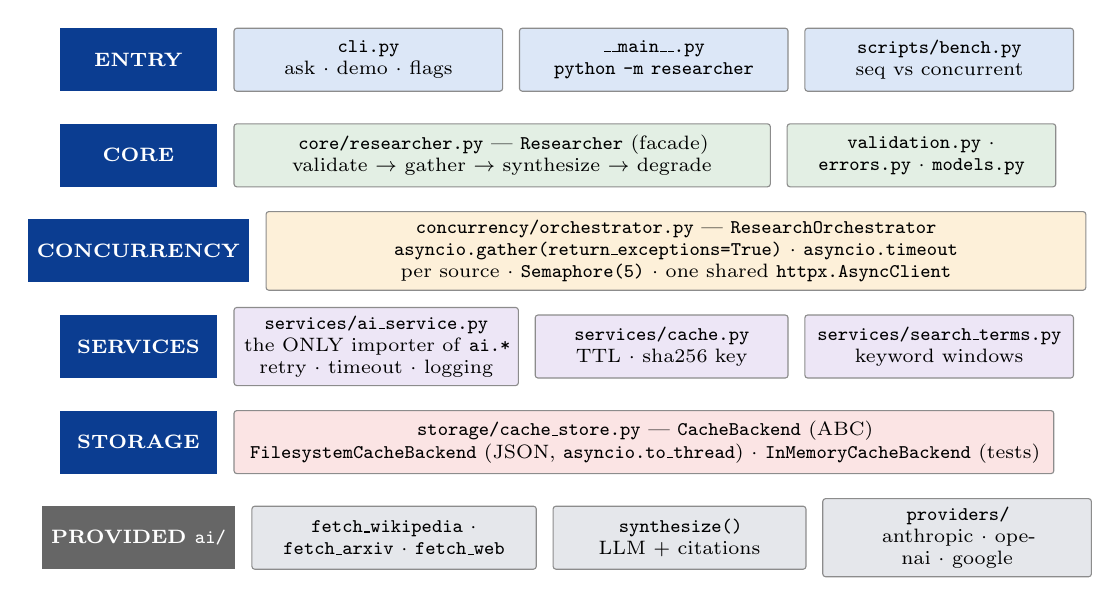
\begin{tikzpicture}[
  font=\scriptsize,
  band/.style={draw=black!45, rounded corners=1pt, minimum height=8mm, align=center, inner sep=3pt},
  lab/.style={draw=none, fill=accent, text=white, font=\scriptsize\bfseries,
              minimum height=8mm, minimum width=20mm, align=center},
  node distance=2mm,
]
\definecolor{cEntry}{HTML}{DCE7F7}
\definecolor{cCore}{HTML}{E3EFE4}
\definecolor{cConc}{HTML}{FDF0D9}
\definecolor{cServ}{HTML}{EDE6F6}
\definecolor{cStor}{HTML}{FBE4E4}
\definecolor{cProv}{HTML}{E5E7EB}

\node[lab] (l1) {ENTRY};
\node[band, fill=cEntry, right=2mm of l1, text width=32mm] (e1) {\texttt{cli.py}\\ ask $\cdot$ demo $\cdot$ flags};
\node[band, fill=cEntry, right=2mm of e1, text width=32mm] (e2) {\texttt{\_\_main\_\_.py}\\ \texttt{python -m researcher}};
\node[band, fill=cEntry, right=2mm of e2, text width=32mm] (e3) {\texttt{scripts/bench.py}\\ seq vs concurrent};

\node[lab, below=4mm of l1] (l2) {CORE};
\node[band, fill=cCore, right=2mm of l2, text width=66mm] (c1)
  {\texttt{core/researcher.py} --- \texttt{Researcher} (facade)\\ validate $\rightarrow$ gather $\rightarrow$ synthesize $\rightarrow$ degrade};
\node[band, fill=cCore, right=2mm of c1, text width=32mm] (c2) {\texttt{validation.py} $\cdot$ \texttt{errors.py} $\cdot$ \texttt{models.py}};

\node[lab, below=4mm of l2] (l3) {CONCURRENCY};
\node[band, fill=cConc, right=2mm of l3, text width=102mm] (o1)
  {\texttt{concurrency/orchestrator.py} --- \texttt{ResearchOrchestrator}\\
   \texttt{asyncio.gather(return\_exceptions=True)} $\cdot$ \texttt{asyncio.timeout} per source $\cdot$ \texttt{Semaphore(5)} $\cdot$ one shared \texttt{httpx.AsyncClient}};

\node[lab, below=4mm of l3] (l4) {SERVICES};
\node[band, fill=cServ, right=2mm of l4, text width=34mm] (s1)
  {\texttt{services/ai\_service.py}\\ the ONLY importer of \texttt{ai.*}\\ retry $\cdot$ timeout $\cdot$ logging};
\node[band, fill=cServ, right=2mm of s1, text width=30mm] (s2)
  {\texttt{services/cache.py}\\ TTL $\cdot$ sha256 key};
\node[band, fill=cServ, right=2mm of s2, text width=32mm] (s3)
  {\texttt{services/search\_terms.py}\\ keyword windows};

\node[lab, below=4mm of l4] (l5) {STORAGE};
\node[band, fill=cStor, right=2mm of l5, text width=102mm] (st1)
  {\texttt{storage/cache\_store.py} --- \texttt{CacheBackend} (ABC)\\
   \texttt{FilesystemCacheBackend} (JSON, \texttt{asyncio.to\_thread}) $\cdot$ \texttt{InMemoryCacheBackend} (tests)};

\node[lab, below=4mm of l5, fill=black!60] (l6) {PROVIDED \texttt{ai/}};
\node[band, fill=cProv, right=2mm of l6, text width=34mm] (p1) {\texttt{fetch\_wikipedia} $\cdot$ \texttt{fetch\_arxiv} $\cdot$ \texttt{fetch\_web}};
\node[band, fill=cProv, right=2mm of p1, text width=30mm] (p2) {\texttt{synthesize()}\\ LLM + citations};
\node[band, fill=cProv, right=2mm of p2, text width=32mm] (p3) {\texttt{providers/}\\ anthropic $\cdot$ openai $\cdot$ google};
\end{tikzpicture}
\end{center}

Dependencies point downward only. The CLI knows about the facade but not about the orchestrator;
the facade knows about the orchestrator but not about \texttt{httpx}; the orchestrator knows about
\texttt{AIService} but not about which LLM is configured. \texttt{bootstrap.build\_researcher()} is
the single composition root --- the only place where concrete implementations are chosen and wired
--- so both the CLI and the benchmark get an identically configured object graph.

\subsection{OOP design \& key abstractions}

The clearest abstraction in our own code is the storage backend, which uses \textbf{inheritance via
an ABC} for substitutability and \textbf{composition} everywhere else.

\begin{lstlisting}[style=python]
class CacheBackend(abc.ABC):
    """Where cache payloads live. Async because the filesystem
    implementation pushes I/O off the event loop."""

    @abc.abstractmethod
    async def read(self, key: str) -> dict | None: ...

    @abc.abstractmethod
    async def write(self, key: str, payload: dict) -> None: ...

    @abc.abstractmethod
    async def delete(self, key: str) -> None: ...
\end{lstlisting}

An ABC is the right tool here because the three methods are a genuine contract with two real
implementations that share no code: \texttt{FilesystemCacheBackend} writes one JSON file per key and
wraps every call in \texttt{asyncio.to\_thread} so blocking disk I/O never stalls the event loop,
while \texttt{InMemoryCacheBackend} is a dict. There is nothing to inherit --- only a shape to agree
on --- which is exactly the case ABCs exist for. Because the tests take the in-memory backend, the
whole suite runs with no filesystem and no cleanup.

Everywhere else we compose rather than inherit. \texttt{SourceCache} \emph{has} a backend rather
than being one --- TTL policy is orthogonal to storage, so mixing them into an inheritance chain
would force a class per (policy $\times$ storage) pair. Likewise \texttt{ResearchOrchestrator}
composes an \texttt{AIService} and a \texttt{SourceCache}, and \texttt{Researcher} composes the
orchestrator. Every one of these is injected through the constructor, which is why the tests can
wire a real object graph and fake only at the \texttt{ai.*} boundary.

\subsection{Data flow across module boundaries}

Our own models are pydantic \texttt{BaseModel}s rather than bare dataclasses, so validation happens
at construction and the same objects serialise straight into the cache payload.

\begin{tabularx}{\textwidth}{@{}lX@{}}
\toprule
\texttt{SourceOutcome} & \texttt{origin}, \texttt{source\_count}, \texttt{error},
\texttt{elapsed\_seconds}, \texttt{from\_cache} --- what happened for one source on one question. \\
\addlinespace
\texttt{ResearchSession} & \texttt{question}, \texttt{answer}, \texttt{outcomes},
\texttt{created\_at}; exposes \texttt{.degraded}, true when any outcome carries an error. \\
\addlinespace
\texttt{Settings} & 18 typed fields via \texttt{pydantic-settings}; validators reject unknown log
levels and non-positive numerics at startup. \\
\bottomrule
\end{tabularx}

\vspace{0.5em}
\begin{deliverbox}
\textbf{No naked dictionaries.} No plain \texttt{dict} crosses a module boundary in our layer. The
one dict in the system is the JSON cache payload, confined to
\texttt{SourceCache}$\leftrightarrow$\texttt{CacheBackend}: built in \texttt{SourceCache.set} and
re-validated back into \texttt{list[Source]} in \texttt{SourceCache.get}, so a corrupted or
schema-drifted file fails loudly at the boundary instead of leaking an untyped mapping upward.
\end{deliverbox}

% =====================================================================
\section{Concurrency \& Performance}\label{sec:concurrency}

\subsection{Why this concurrency model}

We used \textbf{\texttt{asyncio}}. The workload is purely I/O-bound --- three HTTP round trips to
Wikipedia, arXiv and a search API, where essentially all wall-clock time is spent waiting on the
network. Threads would work but cost a stack and a context switch per source for no gain; processes
would be actively wrong, paying interpreter startup and pickling to wait on sockets. The one
genuinely CPU-adjacent call is the synchronous provided \texttt{synthesize()}, which we push off the
loop with \texttt{asyncio.to\_thread} rather than letting it block every other coroutine.

\begin{lstlisting}[style=python]
tasks = [self._run_one(origin, question, use_cache, self._client)
         for origin in requested]
results = await asyncio.gather(*tasks, return_exceptions=True)

async with self._semaphore:                                  # global bound
    async with asyncio.timeout(per_source_timeout_seconds):  # per source
        sources = await fetch(question, max_results=..., client=client)
\end{lstlisting}

Three details matter more than the \texttt{gather} itself. \texttt{return\_exceptions=True} means
one failing source returns an exception object instead of cancelling its siblings --- without it, a
single arXiv outage would take the whole answer down. The timeout is \emph{per task}, not on the
gather, so a slow Wikipedia burns its own budget and not arXiv's. And the semaphore is created once
in the orchestrator's constructor and shared across every question that instance handles, so it
bounds \emph{total} in-flight external calls rather than per-request concurrency --- a per-call
semaphore would bound nothing once several questions run at once, which is exactly what the
benchmark does.

The bound is \texttt{asyncio.Semaphore(MAX\_CONCURRENT\_FETCHES)}, default \textbf{5}. We picked it
from the politeness constraints rather than from our own throughput: the topic brief asks for no
more than about one request per second to arXiv, and Wikipedia rate-limits aggressively. With three
sources per question, 5 lets a single question run fully parallel while keeping a concurrent batch
of five questions from opening fifteen simultaneous connections to three public APIs.

One further optimisation is invisible in the fan-out: the orchestrator owns a \textbf{single
long-lived \texttt{httpx.AsyncClient}}, built at composition time over a process-wide SSL context
cached with \texttt{functools.lru\_cache}. Building the trust store is roughly 0.35\,s and was being
paid per client; hoisting it means connection pooling survives across questions and every client
after the first is nearly free.

\subsection{Sequential-vs-concurrent benchmark}

\texttt{scripts/bench.py} runs the five sample questions from
\texttt{data/research\_questions.json} twice --- once with \texttt{await} in a loop, once through
\texttt{asyncio.gather} --- with caching disabled in both phases so the numbers measure real fetch
and synthesis concurrency rather than cache behaviour. A fresh \texttt{Researcher} is built per
phase so the semaphore and HTTP client do not leak between the two timings.

\vspace{0.4em}
\begin{center}
\begin{tabular}{lccccc}
\toprule
\textbf{Workload} & \textbf{N} & \textbf{Sequential} & \textbf{Concurrent} & \textbf{Speedup} \\
\midrule
5 sample research questions & 5 & 31.4\,s & 8.8\,s & $\mathbf{3.6\times}$ \\
\bottomrule
\end{tabular}
\end{center}
\vspace{0.4em}

\textbf{Run conditions.} Captured 18 September 2026 on Windows 11, Intel 16-core, \textbf{Python
3.13.14}, over a domestic connection. Provider stack: \texttt{LLM\_PROVIDER=anthropic} with
\texttt{claude-sonnet-5}, \texttt{WEB\_SEARCH\_PROVIDER=tavily}. $N = 5$ questions, each fanning out
to three sources. Caching was bypassed in both phases (\texttt{use\_cache=False}). Command:
\texttt{python scripts/bench.py -{}-limit 5}. The raw log is committed at
\texttt{artefacts/bench.md}.

\textbf{Reading the number.} Sequentially the five questions pay 15 source fetches and 5 syntheses
end to end; concurrently the fetches overlap and the five syntheses run together, so total time
collapses towards the slowest single question rather than the sum of all five. It is not $5\times$
because the LLM synthesis step dominates and is itself rate-limited by the provider, and because the
semaphore deliberately caps in-flight fetches at 5.

\subsection{Rate limit \& politeness}

Our strategy is a \textbf{concurrency budget} rather than a token bucket: the shared
\texttt{Semaphore(5)} caps in-flight external calls, and the retry policy's exponential backoff
spreads out anything that does fail. We chose a budget over a rate limiter because the tightest real
constraint here is simultaneous connections to three public APIs, not a published requests-per-second
quota we would have to model.

Backoff is \texttt{tenacity}'s \texttt{wait\_exponential}, configured from \texttt{Settings}:

\begin{lstlisting}[style=python, numbers=none]
wait_exponential(multiplier=RETRY_BACKOFF_SECONDS,
                 min=RETRY_BACKOFF_SECONDS, max=8)
stop_after_attempt(RETRY_MAX_ATTEMPTS)
\end{lstlisting}

\noindent By default that is 3 attempts starting at 0.5\,s and capped at 8\,s. One politeness fix worth recording: Wikimedia rejects generic library
user-agents with a bare 403, so the shared client sends an identifying \texttt{User-Agent} naming
the project and its repository.

\textbf{Highest burst the test suite produces: zero real requests.} Every test is offline by design
--- fakes are injected at the \texttt{ai.*} boundary --- so neither the suite nor CI ever touches a
provider. The highest burst the \emph{application} can produce is 5 concurrent fetches, enforced by
the semaphore.

% =====================================================================
\section{Robustness \& Error Handling}\label{sec:robustness}

\subsection{Wrapping the AI module}

\begin{tabularx}{\textwidth}{@{}lX@{}}
\toprule
\textbf{Retries} & \texttt{tenacity}, scoped to \texttt{ProviderError}, \texttt{httpx.HTTPError},
\texttt{httpx.TimeoutException}. Attempts and backoff come from \texttt{Settings} (default 3 /
0.5\,s, exponential, capped 8\,s), \texttt{reraise=True} so the original exception survives. \\
\addlinespace
\textbf{Not retried} & \texttt{ValueError} --- an empty question or an empty source list is a caller
bug, not a transient fault. Retrying it would turn one fast failure into three slow ones. \\
\addlinespace
\textbf{Timeouts} & Two layers: \texttt{asyncio.timeout(PER\_SOURCE\_TIMEOUT\_SECONDS)} (default
10\,s) around each fetch in the orchestrator, and the same value as the
\texttt{httpx.AsyncClient} transport timeout. \\
\addlinespace
\textbf{Logging} & INFO per call with \texttt{origin}, \texttt{query}, \texttt{results},
\texttt{elapsed}; DEBUG adds titles; WARNING on timeout. \texttt{httpx}/\texttt{httpcore} are pinned
to WARNING. \texttt{print()} is reserved for CLI output. \\
\addlinespace
\textbf{Validation} & Question trimmed and length-checked before any call; origins parsed against a
whitelist; responses re-validated into \texttt{list[Source]} by pydantic. \\
\bottomrule
\end{tabularx}

\subsection{Failure-mode analysis (one concrete incident)}

\textbf{Partial source failure --- one source dies, the answer still ships.}

\begin{itemize}[leftmargin=1.2em, itemsep=2pt]
  \item \textbf{How it was injected.} In \texttt{tests/test\_researcher.py} the arXiv fetcher is
  monkeypatched to raise \texttt{ProviderError} on every attempt, while Wikipedia and web return
  normally. The same path was then exercised for real: \texttt{artefacts/degraded-run.txt} is a live
  run with a deliberately invalid Tavily key.
  \item \textbf{What the system did.} \texttt{gather(return\_exceptions=True)} returned the
  exception instead of cancelling the siblings; the orchestrator turned it into
  \texttt{SourceOutcome(origin=\ldots, source\_count=0, error=\ldots)}; the facade saw a non-empty
  source list and synthesised normally, then appended a degradation note.
  \texttt{session.degraded} is \texttt{True}.
  \item \textbf{What the user saw.} A complete cited answer, followed by
  \texttt{Note: web unavailable (Tavily search failed: Client error '401 Unauthorized' \ldots)} ---
  not a traceback, and not a silently thinner answer.
  \item \textbf{What the logs showed.} INFO lines for the two sources that succeeded with their
  timings, and the retry attempts before the final re-raise.
\end{itemize}

The complement is also tested: when \emph{all} sources fail there is nothing honest to synthesise,
so the facade raises \texttt{NoSourcesAvailableError} listing the failed origins, and the CLI turns
it into a one-line message on stderr with exit code 1.

\subsection{Input validation}

\begin{tabularx}{\textwidth}{@{}p{3.0cm}p{5.2cm}X@{}}
\toprule
\textbf{Entry point} & \textbf{Rule} & \textbf{What the user gets} \\
\midrule
CLI question & non-empty after trim & \texttt{Error: Question must not be empty.} (exit 1) \\
CLI question & $\le$ \texttt{MAX\_QUESTION\_LENGTH} & \texttt{Error: Question too long (N > 500 characters).} \\
\texttt{-{}-sources} & \texttt{wiki|wikipedia|arxiv|web} & \texttt{Error: Unknown source 'x'; expected one of \ldots} \\
\texttt{LOG\_LEVEL} & a valid level name & \texttt{ValidationError} at startup, naming the field \\
numeric env vars & must be positive & \texttt{ValidationError} at startup, before any network call \\
provider responses & re-validated to \texttt{list[Source]} & malformed payload fails at the boundary \\
cache files & JSON-decoded defensively & a corrupt file is a miss, never a crash \\
\bottomrule
\end{tabularx}

\vspace{0.4em}
Two deliberate choices. Configuration is validated at \emph{startup} rather than at first use, so a
typo in \texttt{.env} fails immediately instead of thirty seconds into a demo. And every error the
user can cause surfaces as a single line on stderr with exit code 1 --- the CLI catches
\texttt{ResearcherError}, the base of our own exception hierarchy, so a bare traceback never reaches
the terminal.

% =====================================================================
\section{Storage \& Caching}\label{sec:storage}

\subsection{Schema}

\begin{deliverbox}
\textbf{Why there is no SQLite schema.} The brief allows PostgreSQL, filesystem JSON or in-memory
for the cache, and we chose \textbf{filesystem JSON}. The only thing worth persisting here is
\texttt{(source, query)} $\rightarrow$ \texttt{list[Source]}: there are no relations, no queries
beyond an exact key lookup, and no reporting. A relational schema would add a dependency and a
running service to support a key--value read. Swapping in PostgreSQL later means one new
\texttt{CacheBackend} subclass and one line in \texttt{bootstrap.py} --- which is the point of the
ABC.
\end{deliverbox}

\vspace{0.4em}
The on-disk payload is one JSON document per key:
\texttt{source}, \texttt{query} (canonicalised), \texttt{cached\_at}, \texttt{expires\_at}, and
\texttt{sources} (the serialised \texttt{list[Source]}). \texttt{cached\_at} and \texttt{expires\_at}
are derived; the \texttt{sources} array is the source of truth. The key itself is
\texttt{sha256("\{source\}:\{canonical query\}")}, which is both the filename and the index.

\subsection{Caching policy}

\begin{tabularx}{\textwidth}{@{}lX@{}}
\toprule
\textbf{What} & Raw \texttt{list[Source]} per source, \emph{not} the synthesised answer --- LLM
output is not deterministic per call, and the brief asks for source-level caching. \\
\addlinespace
\textbf{Key} & \texttt{sha256("\{source\}:\{canonical query\}")}; canonicalisation lowercases,
strips and collapses whitespace, so \texttt{"WHAT IS   Photosynthesis?"} and
\texttt{"what is photosynthesis?"} share one entry. \\
\addlinespace
\textbf{Where} & One JSON file per key under \texttt{CACHE\_DIR} (default \texttt{./.cache}), all
I/O via \texttt{asyncio.to\_thread}. \\
\addlinespace
\textbf{How long} & \texttt{CACHE\_TTL\_SECONDS}, default 86400 (24\,h). \\
\addlinespace
\textbf{Invalidation} & Lazy expiry --- a read past \texttt{expires\_at} is reported as a miss and
refetched. No sweeper process; \texttt{-{}-no-cache} bypasses both read and write. \\
\addlinespace
\textbf{Ordering} & The cache is checked \emph{before} the semaphore is acquired, so a cache hit
never consumes a concurrency slot. This is pinned by a test. \\
\bottomrule
\end{tabularx}

\vspace{0.5em}
\textbf{Measured hit rate.} From \texttt{artefacts/cache-hit.txt}, the same question asked twice
against a clean \texttt{.cache}: \textbf{0/3 hits cold, 3/3 hits warm}. Per-source fetch time fell
from \texttt{wikipedia=0.43s, arxiv=0.40s, web=3.86s} (4.69\,s total) to \texttt{0.02s} each --- a
$78\times$ reduction on the retrieval half of the request. Synthesis is deliberately not cached, so
the second run still pays the LLM call.

% =====================================================================
\section{Testing}\label{sec:testing}

\subsection{Strategy \& coverage}

\textbf{90 tests, 95\,\% statement coverage, and not one of them touches the network.} Coverage is
enforced in CI with \texttt{-{}-cov-fail-under=60}; we are comfortably above it. The provided
\texttt{tests/test\_ai\_smoke.py} is unmodified and all 16 of its tests still pass.

\vspace{0.4em}
\begin{center}\small
\begin{tabular}{lrrr}
\toprule
\textbf{Module} & \textbf{Stmts} & \textbf{Miss} & \textbf{Cover} \\
\midrule
\texttt{services/ai\_service.py}        & 55 & 0 & 100\,\% \\
\texttt{services/cache.py}              & 25 & 0 & 100\,\% \\
\texttt{services/search\_terms.py}      & 15 & 0 & 100\,\% \\
\texttt{core/researcher.py}             & 31 & 0 & 100\,\% \\
\texttt{models.py} $\cdot$ \texttt{core/errors.py} & 26 & 0 & 100\,\% \\
\texttt{concurrency/orchestrator.py}    & 68 & 1 & 99\,\% \\
\texttt{cli.py}                         & 74 & 1 & 99\,\% \\
\texttt{config.py}                      & 43 & 2 & 95\,\% \\
\texttt{storage/cache\_store.py}        & 49 & 3 & 94\,\% \\
\texttt{core/validation.py}             & 25 & 2 & 92\,\% \\
\midrule
\textbf{TOTAL}                          & \textbf{435} & \textbf{22} & \textbf{95\,\%} \\
\bottomrule
\end{tabular}
\end{center}

\vspace{0.4em}
\textbf{How we mocked.} Fakes are injected at exactly one seam --- the \texttt{ai.*} functions ---
using \texttt{monkeypatch} against \texttt{ai\_service\_module.ai\_sources} and \texttt{ai\_synth}.
Everything below that seam is the real object graph: a real \texttt{ResearchOrchestrator}, a real
\texttt{SourceCache} over \texttt{InMemoryCacheBackend}, a real \texttt{AIService} with its real
retry policy. That is deliberate: mocking the orchestrator would have meant testing our mocks
instead of our wiring. \texttt{respx} is available for the HTTP layer, and the provided smoke tests
additionally block outbound sockets.

\subsection{Notable tests}

\begin{itemize}[leftmargin=1.2em, itemsep=3pt]
  \item \textbf{Happy path, end to end.}
  \texttt{test\_ask\_happy\_path\_returns\_session\_with\_citations} wires the full graph, asks a
  question, and asserts that all three origins appear in \texttt{outcomes}, that citations came
  back, and that \texttt{degraded} is \texttt{False}. It is the test that would catch a
  composition-root mistake.
  \item \textbf{Concurrency.} \texttt{tests/test\_orchestrator.py} asserts that when one task raises,
  \texttt{gather} still returns the others; that a slow source trips its own \texttt{asyncio.timeout}
  without touching its siblings; that the semaphore's observed peak never exceeds the configured
  bound; and that a cache hit is served before the semaphore is acquired.
  \item \textbf{Error path that caught a real bug.}
  \texttt{test\_ask\_prints\_non\_latin1\_characters\_to\_a\_redirected\_stream}. Answers contain
  characters Windows' legacy code page cannot encode; with output redirected, printing them raised
  \texttt{UnicodeEncodeError} \emph{mid-answer}, after the user had already seen half of it. The CLI
  now reconfigures stdout to UTF-8, and the test pins both that and the case where the stream cannot
  be reconfigured at all.
\end{itemize}

% =====================================================================
\section{Deployment \& Reproducibility}\label{sec:deploy}

\subsection{Docker image}

\begin{lstlisting}[style=python, numbers=none, language=bash]
$ docker build -t research-assistant .
$ docker run --rm --env-file .env research-assistant
$ docker run --rm --env-file .env research-assistant ask "What is photosynthesis?"
$ docker run --rm research-assistant pytest tests/test_ai_smoke.py -v
\end{lstlisting}

\textbf{Single-stage} build on \texttt{python:3.12-slim}. A multi-stage build buys little here:
there is no compile step and no build-time toolchain to discard, so the only saving would be pip's
cache, which \texttt{-{}-no-cache-dir} already prevents. \texttt{requirements.txt} is copied and
installed before the source so the dependency layer stays cached across code edits. The container
runs as a non-root \texttt{appuser} that owns \texttt{/app/.cache}, and the default \texttt{CMD}
runs the five-question demo. The built image is \textbf{472\,MB}, almost all of it the \texttt{python:3.12-slim} base and the installed wheels.

CI (\texttt{.github/workflows/ci.yml}) runs four jobs on every pull request and every push to
\texttt{main}: \textbf{ruff} lint, \textbf{mypy} type check over \texttt{researcher/},
\textbf{pytest with the coverage gate}, and a \textbf{Docker build} that then runs
\texttt{python -m researcher -{}-help} inside the image to prove the entry point is wired.
Superseded runs on the same branch are cancelled rather than paid for twice. No API keys are present
in CI --- by design, since every test is offline.

\subsection{Configuration}

\begin{center}\small
\begin{tabularx}{\textwidth}{@{}>{\RaggedRight\arraybackslash}p{5.1cm}
                              >{\RaggedRight\arraybackslash}p{2.3cm} X@{}}
\toprule
\textbf{Variable} & \textbf{Default} & \textbf{If missing / invalid} \\
\midrule
\texttt{LLM\_PROVIDER} & \texttt{anthropic} & default used; an unknown value raises
\texttt{ProviderError} at the first synthesis \\
\addlinespace
\texttt{LLM\_MODEL} & \emph{unset} & the provider SDK's own default model id is used \\
\addlinespace
\texttt{ANTHROPIC\_API\_KEY} /\newline
\texttt{OPENAI\_API\_KEY} /\newline
\texttt{GOOGLE\_API\_KEY} &
\emph{none} & the one matching \texttt{LLM\_PROVIDER} is required; missing
$\to$ \texttt{ProviderError} from the factory, retried 3$\times$, so the \texttt{ask}
fails \emph{after} fetching \\
\addlinespace
\texttt{WEB\_SEARCH\_PROVIDER} & \texttt{tavily} & default used; an unknown value degrades
the web source \\
\addlinespace
\texttt{TAVILY\_API\_KEY} /\newline
\texttt{SERPER\_API\_KEY} & \emph{none} &
required for the matching provider; missing $\to$ the web source is reported unavailable
and the answer is still produced from Wikipedia and arXiv \\
\addlinespace
\texttt{LOG\_LEVEL} & \texttt{INFO} & default used; an invalid level raises
\texttt{ValidationError} at start-up \\
\texttt{CACHE\_DIR} & \texttt{./.cache} & default used; created on first write \\
\texttt{CACHE\_TTL\_SECONDS} & \texttt{86400} & default (24\,h); $\le 0 \to$ \texttt{ValidationError} \\
\texttt{PER\_SOURCE\_TIMEOUT\_SECONDS} & \texttt{10} & default (10\,s); $\le 0 \to$ \texttt{ValidationError} \\
\texttt{MAX\_SOURCES\_PER\_QUERY} & \texttt{3} & default; $\le 0 \to$ \texttt{ValidationError} \\
\texttt{MAX\_CONCURRENT\_FETCHES} & \texttt{5} & default; $\le 0 \to$ \texttt{ValidationError} \\
\texttt{MAX\_QUESTION\_LENGTH} & \texttt{500} & default; $\le 0 \to$ \texttt{ValidationError} \\
\texttt{RETRY\_MAX\_ATTEMPTS} & \texttt{3} & default; $\le 0 \to$ \texttt{ValidationError} \\
\texttt{RETRY\_BACKOFF\_SECONDS} & \texttt{0.5} & default (0.5\,s); $\le 0 \to$ \texttt{ValidationError} \\
\bottomrule
\end{tabularx}
\end{center}

\vspace{0.4em}
Every one of these has a working default except the API keys, so \texttt{python -m researcher
-{}-help} and the whole test suite run on a machine with no \texttt{.env} at all. \texttt{Settings}
sets \texttt{extra="ignore"} so an unrelated key in \texttt{.env} does not crash startup.

% =====================================================================
\section{Limitations \& Future Work}\label{sec:limits}

\begin{itemize}[leftmargin=1.2em, itemsep=3pt]
  \item \textbf{The search-term fallback is a heuristic, not a fix.} Reshaping a question into
  keyword windows makes Wikipedia return \emph{something}, but it is a stopword list and a sliding
  window tuned against five sample questions. A question whose topic word is also a stopword will
  still do badly. The honest fix is a different Wikipedia endpoint, which the contract does not let
  us reach.
  \item \textbf{Cache keys ignore \texttt{max\_results}.} Asking for 3 sources and later for 10 hits
  the same entry and silently returns 3. Nothing in the CLI exposes that knob today, so it cannot
  bite yet --- but it is a latent bug, not a design decision.
  \item \textbf{No persistence beyond the cache.} A \texttt{ResearchSession} is built, printed and
  dropped. Storing sessions would make the tool answerable to ``what did we ask last week''.
  \item \textbf{The concurrency bound is global, not per-host.} One semaphore covers Wikipedia,
  arXiv and the search provider together, so a slow arXiv can hold slots Wikipedia could have used.
  \item \textbf{With another week} we would add a per-host rate limiter, persist sessions, and
  replace the keyword heuristic with a proper search strategy --- in that order, because that is the
  order in which they change what a user experiences. Re-running the benchmark on a quieter network
  would also tighten the number: the $3.6\times$ above was measured over a domestic connection, so
  the sequential leg carries some noise.
\end{itemize}

% =====================================================================
\section{Tools \& Acknowledgements}\label{sec:tools}

The team used \textbf{Claude Code} throughout. Design decisions --- the layering, the single
\texttt{ai.*} choke point, the cache key scheme, the slicing of work into reviewable pull requests
--- were made by the team before any code was generated, and every pull request was reviewed by a
second member before it landed.

\begin{center}\small
\begin{tabularx}{\textwidth}{@{}lXl@{}}
\toprule
\textbf{Area} & \textbf{Assistant} & \textbf{Reviewed} \\
\midrule
\texttt{config.py}, \texttt{models.py}, validation (\#1) & Claude Code & PR \#1 \\
\texttt{cache.py}, \texttt{cache\_store.py} (\#2) & Claude Code & PR \#2 \\
\texttt{ai\_service.py}, \texttt{search\_terms.py} (\#3) & Claude Code & PR \#3 \\
\texttt{orchestrator.py}, facade, bootstrap (\#4) & Claude Code & PR \#4 \\
\texttt{cli.py}, \texttt{bench.py} (\#5) & Claude Code & PR \#5 \\
Test suite (\#6--\#9) & Claude Code & each PR reviewed \\
Dockerfile, CI, linter config (\#10) & Claude Code & PR \#10 \\
README (\#11) & Claude Code & PR \#11 \\
Live-run artefacts (\#12) & captured from a real run & PR \#12 \\
Benchmark citation in the README (\#13) & Claude Code & PR \#13 \\
\texttt{COMMON\_PITFALLS} audit fixes (\#14) & Claude Code & PR \#14 \\
This report (\#15) & LaTeX from the course template & PR \#15 \\
Slide deck (\#16) & Beamer from the course template & PR \#16 \\
Final tag \& submission (\#17) & --- & PR \#17 \\
\bottomrule
\end{tabularx}
\end{center}

\vspace{0.6em}
\textbf{Contribution statement.} All work landed through pull requests, each reviewed by a teammate
before merge. Seventeen pull requests, split 6 / 6 / 5:

\begin{center}\small
\begin{tabularx}{\textwidth}{@{}llXc@{}}
\toprule
\textbf{Member} & \textbf{GitHub} & \textbf{Pull requests} & \textbf{Share} \\
\midrule
Sanan Garibli & \texttt{@sanan-garibli} & \#1 config \& models $\cdot$ \#4 orchestrator \& facade $\cdot$ \#7 AIService tests $\cdot$ \#10 Docker \& CI $\cdot$ \#17 final tag \& submission & 5/17 \\
\addlinespace
Humbat Camalov & \texttt{@Camalzadeh} & \#3 AIService \& search terms $\cdot$ \#5 CLI \& benchmark $\cdot$ \#9 facade \& CLI tests $\cdot$ \#12 live-run artefacts $\cdot$ \#14 pitfall audit fixes $\cdot$ \#16 slide deck & 6/17 \\
\addlinespace
Farah Nematzada & \texttt{@f4r4hh} & \#2 cache \& storage $\cdot$ \#6 config/cache/storage tests $\cdot$ \#8 orchestrator tests $\cdot$ \#11 README $\cdot$ \#13 benchmark citation $\cdot$ \#15 this report & 6/17 \\
\bottomrule
\end{tabularx}
\end{center}

% ===== REFERENCES ====================================================
\section*{References}
\addcontentsline{toc}{section}{References}

\begin{enumerate}[label={[\arabic*]},leftmargin=2.4em,itemsep=2pt]
  \item Python Software Foundation, \emph{asyncio --- Coroutines and Tasks}:
  \texttt{gather}, \texttt{timeout}, \texttt{Semaphore}, \texttt{to\_thread}.
  \url{https://docs.python.org/3/library/asyncio-task.html}
  \item J.~Kirkland et al., \emph{Tenacity} retrying library documentation --- retry
  policies and \texttt{wait\_exponential}. \url{https://tenacity.readthedocs.io/}
  \item Encode, \emph{HTTPX} documentation --- \texttt{AsyncClient}, connection pooling
  and timeouts. \url{https://www.python-httpx.org/async/}
  \item Pydantic, \emph{pydantic-settings} documentation --- environment-backed settings
  and the \texttt{extra} policy. \url{https://docs.pydantic.dev/latest/concepts/pydantic_settings/}
  \item Anthropic, \emph{Claude API documentation} --- models and rate limits
  (\texttt{LLM\_PROVIDER=anthropic}, \texttt{claude-sonnet-5}).
  \url{https://docs.anthropic.com/}
  \item Tavily, \emph{Search API documentation} --- the default
  \texttt{WEB\_SEARCH\_PROVIDER}. \url{https://docs.tavily.com/}
  \item Wikimedia Foundation, \emph{User-Agent policy} --- why the shared client sends an
  identifying header. \url{https://meta.wikimedia.org/wiki/User-Agent_policy}
  \item arXiv, \emph{API User's Manual: rate limiting and terms of use}.
  \url{https://info.arxiv.org/help/api/tou.html}
  \item \emph{RESPX} --- \texttt{httpx} mocking, and \emph{pytest-asyncio}; together these
  keep all 90 tests offline. \url{https://lundberg.github.io/respx/}
  \item AI Academy, \emph{Topic 4 --- Async Research Assistant} (\texttt{TOPIC.md}),
  \texttt{docs/GIT\_WORKFLOW.md} and \texttt{docs/COMMON\_PITFALLS.md}; team repository
  \repolink, tag \texttt{v1.0-final}.
\end{enumerate}

% ===== APPENDIX ======================================================
\section{Appendix --- Reproducing the benchmark}

\begin{lstlisting}[style=python, numbers=none, language=bash]
git clone https://github.com/team-M503-SWE-06/research-assistant
cd research-assistant
python -m pip install -r requirements.txt
cp .env.example .env        # then fill in an LLM key and a web-search key
python scripts/bench.py --limit 5
\end{lstlisting}

The committed output of exactly this command, together with a full demo run, a single question,
cold-versus-warm cache behaviour and a deliberately degraded run, is under \texttt{artefacts/} in
the repository.

\end{document}
